% Preamble
% ---
\documentclass[12pt]{article}

% Packages
% ---
\usepackage{amsmath} % Advanced math typesetting
\usepackage[utf8]{inputenc} % Unicode support (Umlauts etc.)
\usepackage{hyperref} % Add a link to your document
\usepackage{graphicx} % Add pictures to your document
\usepackage{listings} % Source code formatting and highlighting
\usepackage[left=2.5cm, right=2.5cm, top=2.5cm]{geometry}
% Main document
% ---
\begin{document}


% Set up the maketitle command
\author{Tolga Atabas}
\title{\includegraphics[width=0.4\textwidth]{swarthmore_logo.jpg} \\ COVID-19 Data Analysis in Delaware \\ Summer Research Project}
\date{July 18, 2020}

\maketitle{} % Generates title
\tableofcontents{} % Generates table of contents from sections

\thispagestyle{empty}
\clearpage
\setcounter{page}{1}

\section{Abstract}
\paragraph{}
The COVID-19 pandemic has impacted this country’s public health, education, and economic wellbeing in many ways. Schools were closed, the economy was shut down, and mask wearing was instituted. The purpose of this study was to quantitatively take a look at the changes in cases of COVID-19 patients as the pandemic progressed. Exponential models were fitted for both the cumulative cases and daily cases data for the State of Delaware. Important policy dates are also considered during data analysis. Thus, it is possible to relate any falls or rises in the exponential model parameters to policies or social activites occurring within that corresponding time period.
\vspace{3cm}
\begin{figure}[h]
\centering
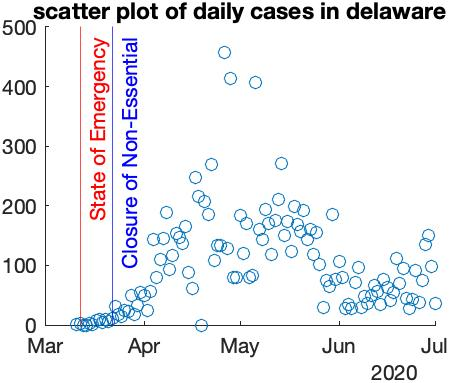
\includegraphics[width=0.4\textwidth]{Figure1.jpg}
\caption{A scatterplot of the daily cases encountered in Delaware from its first cases on March 11, 2020 to the most recent day from the date of the creation of the figure which was June 23, 2020. This is intended to give a beginning understanding to what the project aims to do by showing that the data is visualized by looking at the real data and overlaying important dates of policies and also model calculations later on.}
\end{figure}

\pagebreak

\section{Introduction}
\praragraph{} This project began as a hands-on introduction to modeling real data to mathematical models. However, with the COVID-19 pandemic, it was possible to transition the project's goal to modeling data from this modern occurrence. Analyzing this data with quantitative methods allows for a better understanding of the relationship between the progression of the pandemic and policies taken by those in power. The COVID-19 pandemic has impacted this country’s public health, education, and economic wellbeing in many ways. Schools were closed, the economy was shut down, and mask wearing were instituted. There was empirical evidence that such measures would have a desired impact, but there is quantification of what that impact might be. The purpose of this study was to take data from a small section of society and use this data from case counts to determine what, if any, impact these decisions might have. The data for the state of Delaware was taken for this study. It is a small self-contained community which experienced significant impact from the virus.
\paragraph{} Several different models were applied to the data and the models were evaluated to determine which was most appropriate. The parameters in the model were indicative of a change in policy and its effectiveness. Due to the highly infective nature of the virus, exponential models of forms $y = ae^{kt} \textnormal{ and } y = ae^{kt} + b$ were used. More information will be provided as to why two models were used, and the advantages or disadvantages of each.
\paragraph{} After an appropriate model was determined, comparisons were made to the data shown in the various figures and the policies that were enacted by the Governor of Delaware, John Carney. The State of Delaware keeps a \href{https://governor.delaware.gov/health-soe/}{record of all actions^1} that the State took in response to the pandemic. The data, which was acquired from a \href{https://github.com/nytimes/covid-19-data/blob/master/us-states.csv}{New York Times GITHUB Repository^2}, was interpretted in the scope of these policies.
\paragraph{} Additionally, to understand the modeling methods in this study it is important to have a working knowledge of MATLAB, especially the \href{https://www.mathworks.com/help/optim/ug/fmincon.html}{fmincon^3} function from the Opimization Toolbox. An understanding of linear algebra and least squared data fitting is also necessary, as well as an introductory understanding in statistics.
\paragraph{} All code, figures, and functions can be found on my \href{https://github.com/tatabas/delaware-covid-analysis}{GITHUB Repository^4} at \url{https://github.com/tatabas/delaware-covid-analysis}.

\section{Methods \& The Model}
\paragraph{} The first step in starting the analysis was to obtain the data from the \href{https://github.com/nytimes/covid-19-data/blob/master/us-states.csv}{New York Times GITHUB Repository^2} which lists the cumulative cases in each state per day. After acquiring this data, it was simple enough to extract the data for Delaware only and then begin the analysis.
\paragraph{} The structure of this section will be set as follows: the methods of analysis for the cumulative cases data will be explained first. This analysis was done with two models: $y = ae^{kt} \textnormal{ and } y = ae^{kt} + b$. After an in depth review of the modeling methods employed in this project for the cumulative data, daily data will be explained in a similar manner. Daily data was only modeled using $y = ae^{kt}$.

\subsection{Cumulative Data: y = ae ^{kt}}
\paragraph{} It was appropriate to use a basic exponential function to begin a quantitative search into the present data set. Since the virus has a very infective nature, an exponential model would be able to capture the fast-paced compounded growth. Before going into the mathematics, it is worth taking note on the logic behind the model.
\paragraph{} The logic of the model assumes that the model parameters do not change in a span of 14 days. This is why each modeling window is 14-days in length. Each modeling window consists of a constant set of time (t) values 0 to 13, [0:13], and the COVID-19 case (y) values for that window of time. Then, the next modeling window is created by shifting over one day. For example, the t vector for the first modeling window is [0:13] and the y vector is made up of the COVID-19 cases for days [1:14] of the pandemic in Delaware. Then the second modeling window has a t vector [0:13] again and the y vector is the case values for days [2:15]. This method allows for the viewing of changes in the infection rate as the virus progresses.
\paragraph{} Before moving forward, it is worth clearing some other aspects of this model. One aspect being that a modeling window of 7 days was attempted initially, but the resulting data created too much noise that it was not possible to interpret actual changes in infection rate to noise from a small data set in a short modeling window. Another aspect being that the t vector is a constant [0:13] because if it were to change with the day number (e.g [1:14] and then [2:15]) then the modeling would be inconsistent since higher t values would decrease/change the values of the parameters being calculated. It was decided that 0 was a proper point to start the vector because it makes the system neater: $y = ae ^ {kt} = ae^{0} = a$. Also, this model is reflected in \href{https://github.com/tatabas/delaware-covid-analysis}{firstmodelCumulativeDelaware.m} in my GITHUB Repository.
\begin{figure}[h]
  \centering
  \subfigure[a]{%
    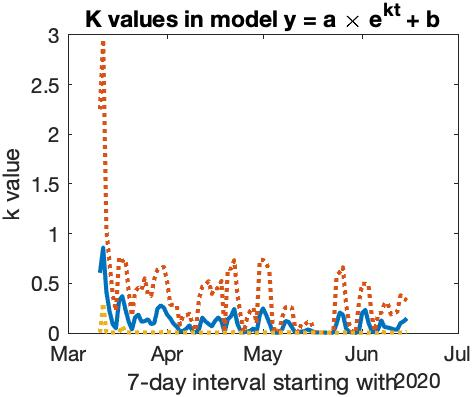
\includegraphics[width=0.4\textwidth]{Figure2a.jpg}%
    \label{fig:a}%
  }%
  \hfill
  \subfigure[b]{%
    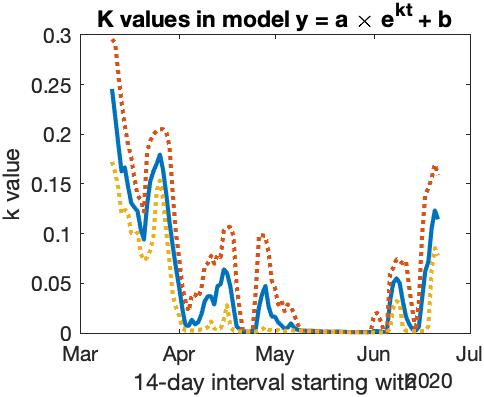
\includegraphics[width=0.4\textwidth]{Figure2b.jpg}%
    \label{fig:b}%
  }%
  \caption{Plot A shows the k parameters in the $y = ae^{kt} +b$ model under the 7-day modeling window, whereas plot B shows it under the 14-day modeling window. The dashed lines represent the upper and lower bounds of the 95\% confidence intervals for the model. Since the 7-day modeling window resulted in calculations that have wide ranges in the confidence interval and lots of suddent drops, the 14-day modeling window was deemed more appropriate. The 7-day modeling window does not provide much valuable information due to the noise created by sudden drops and rises. More will be explained as to how the data in these figures were calculated.}
  \label{fig:2}
\end{figure}
\paragraph{} Now, it is possible to start the explanation of how the y vector was fit to the $y = ae^{kt}$ model. Since this is a simple model, methods from linear algebra were utilized to begin the data fitting process. The natural log (base e) was taken to linearize the equation, resulting in $log(y) = log(a) + kt$. Using this model, it is possible to get to the linear algebra model where there is a matrix A (a 14X2 matrix composed of a column of ones paired with the t vector, [0:13]), a vector p (made up of the parameters a and k), and a vector y (made by taking the log of cases data) $Ap = y$. Solving for p: $ p = (A^T A)^{-1}  A^T  y$. With this method, it is possible to get the parameters for the specified window. At the time of this analysis, the available data consisted of cases up to and including July 18th. Thus, there were 117 modeling windows, producing 117 sets of parametes.
\paragraph{} After establishing an understanding of the 14-day window modeling structure, it is necessary to cover another calculation that was utilized. Each modeling window was \href{https://www.mathworks.com/help/stats/bootstrp.html}{bootstrapped^5} to get a probability distribution for the parameters of each modeling window. The purpose of running a bootstrapping program was to create a probability distribution to express the 95\% confidence interval to understand the relative uncertainty for the parameters. The bootstrapping function works as follows: it takes a random sample of size 14 with replacement from the vector t and y 1000 times and then sends this randomized sample to the model fitting function explained above.
\paragraph{} Before progressing from this point, it was important to verify that the randomization did not affect the calculation of the parameters. The simplest way to check this was to do a simple randomized test as follows:
\begin{lstlisting}
%making sure that random orders return the same values

%first set of variables in original order
%second set of variables have y in ascending and t in descending order
y = log(delaware.cases(1:14));
t = [0:13]';
%a randomized t variable
t_r =[3 7 1 5 8 12 2 0 13 9 4 10 6 11]';
%a y variable that is randomized with same indices
%adding one because the range of t is 0:6, needs to fit 1:7 index of y
y_r = y(t_r+1);

%finding constants for original set of data
A = [ones(14,1),t];
p = inv(A'*A)*A'*y;
a = exp(p(1));
k = p(2);

%finding constants for data with different order
A_r = [ones(14,1),t_r];
p_r = inv(A'*A)*A'*y_r;
a_r = exp(p_r(1));
k_r = p_r(2);
\end{lstlisting}
After running this test it was possible to determine by comparing $a,a_r$ and $k,k_r$ that the randomization did not have a negative impact on calculation. This provided the necessary proof to be able to continue with the process and trust that bootstrapping would not create incorrect values.
\paragraph{} As can be assumed, the result from adding a bootstrapping function to the 117 modeling windows results in two matrices of size 1000X117. One matrix is for the parameter $a$ and the other for parameter $k$ in the model $y = ae^{kt}$. Before accepting these results, the means and medians of the bootstrapped results for each modeling window were compared to the non-bootstrapped results of that window. All of these results were close in value, showing that the probability distribution was relatively normal and accurate. Therefore, the mean was taken as the calculated parameter value and the 25th and 975th points (after sorting from least to greatest) were taken as the lower and upper bounds, respectively, for the 95\% confidence interval.
\paragraph{} After going through these methods, it was possible to simply plot the values and acquire a visual representation of the changes in parameters for each modeling window with their corresponding 95\% error bars.

\subsection{Cumulative Data: y = ae ^ {kt} + b}
\paragraph{} As should be expected, the policy changes enacted by the Governor's office in Delaware caused changes in cases. In terms of modeling, these extreme drops in cases from effective policies or extreme rises in cases from outbreaks cannot be captured by the previous model. However, an additional $+b$ parameter allows for these changes to be reflected in the analysis. And it is for this reason that the $y = ae ^ {kt} + b$ model was introduced. The logic from the previous model applies to this regarding the 14-day modeling windows.
\paragraph{} Because of the additional $+b$ parameter, it was no longer possible to use the linear algebra methods used in the previous model. Instead, the \href{https://www.mathworks.com/help/optim/ug/fmincon.html}{fmincon^3} function was used to find the model that optimizes, or decreses, the distance between the observed and calculated values, effectively finding the least squares error.
\paragraph{} As explained before, the calculation for modeling is conducted for each 14-day modeling window. There are 117 modeling windows for this method as of July 18,2020, the date for which this report is based upon. For each modeling window, the t vector was a constant [0:13] and the y vector was the cases data for the corresponding 14-day window. There was no need to take the log of these values because log is not used for linearization in this method.
\paragraph{} Fmincon is a function that optimizes – minimizes – an objective function. The objective function in this situation is a function that calculates least squares errors. By setting the objective function of fmincon as the least squares error, it is possible to minimize the error between the actual cases data and the model that is created. To illustrate how this works, it is best to show a code piece:
\begin{lstlisting}
if day == 1
  %the initial point is in form [a;k;b]. 1.9 and 0.3 come from the
  %first model which was based upon y = ae^kt. It serves as an
  %approporiate starting point for this analysis.
p(day,:) = fmincon(@(x)lstSqrs(x,t,y),[1.9;0.3;0],[],[],[],[],[-inf;0;-inf],
  [inf;20;inf]); %[a k b]
%a and b can be negative due to policies that heed the growth of virus
%k is always positive because cumulative data cannot have negative growth
else
%the parameters for the previous window make an approporate guess
p(day,:) = fmincon(@(x)lstSqrs(x,t,y),[p(day-1,1);p(day-1,2);p(day-1,3)],
  [],[],[],[],[-inf;0;-inf],[inf;20;inf]);
end
\end{lstlisting}
\paragraph{} This is a fairly complex piece of code, however the first note that should be made is regarding the structure of fmincon. Fmincon starts with a function as the first input. An implicit in-line function was created, as seen in the code, to create a variable for the guesses that the fmincon tries as it searches for the optimized value. The second input is the initial guessing point. For this program, the first guess came from the first modeling window in the previous model, $y = ae ^ {kt}$. Since the first modeling window in the previous model had $a = 1.9$ and $k = 0.3$, the initial guess for the first week in this model was $a = 1.9$, $k = 0.3$, and $b = 0$. The following brackets can be filled in with values for linear constraints, but no constraints were used in this calculation. The last two inputs are the limits for each parameter. Parameters $a$ and $b$ were left without a bound because they could be negative or positive depending on the cases of that modeling window. Since $k$ did not exceed 5, it was appropriate to leave the upper bound at 20.
\paragraph{} In order to continue making an educated guess about the initial starting point for the fmincon function, each subsequent fmincon calculation used the calculated parameters from the previous modeling window as the initial guess. This allowed for consistency and accuracy in the calculations since the parameters are not expected to change extremely between two adjacent modeling windows.
\paragraph{} The lstSqrs function inputted to the fmincon function is a custom function that was created to take the fmincon inputs of x and model plug them into the equation $y = x(1)e ^ {x(2)t} +x(3)$ (because fmincon sends a vector x with [a k b] order). Then it finds the sum of squared error between this equation and the real data. After finding the set of parameters that minimizes the sum of squared errors, this set of parameters is sent back as the answer, which is recorded.
\paragraph{} As was done previously, bootstrapping was also added to this function to get a sense of the amount of error in the calculations. To follow the same thought track as before, the code for testing effects of randomization will be expressed in the same way:
\begin{lstlisting}
t = [1:7];
y = delaware.cases(1:7);
t_r = [1,2,7,3,4,5,6]; %need to scramble same set of data
y_r = y(t_r);
t_r(7)=6;
y_r(7)=8;

c = fmincon(@(x)lstSqrs(x,t,y),[1.7;0.3;0],[],[],[],[],[-inf,0,-inf],
  [inf,20,inf]);
c_r = fmincon(@(x)lstSqrs(x,t_r,y_r),[1.7;0.3;0],[],[],[],[],[-inf,0,-inf],
  [inf,20,inf]);
\end{lstlisting}
After running this test it was possible to determine by comparing $c,c_r$ that the randomization did not have a negative impact on calculation. This provided the necessary proof to be able to continue with the process and trust that bootstrapping would not create incorrect values.
\paragraph{} The bootstrapping was done in a similar way: random sample with replacement was taken from vectors t and y 1000 times, each time the randomized order was plugged into the fmincon function, then following the coding path to the lstSqrs function to find the best model to fit that set of data. In the same way, the mean of each modeling window's bootstrapped data was accepted as the calculated parameter, and the 25th and 975th points as the bounds for the 95\% confidence interval. The code for this model can be found under the MATLAB code named \href{https://github.com/tatabas/delaware-covid-analysis}{finalCumulativeDelaware.m}

\subsection{Daily Data: y = ae ^ {kt}}
\paragraph{} After finishing calculations on the cumulative data with the two models, the focus was shifted towards the the daily data. In order to get the daily data from the cumulative data in the NYT GITHUB Repository, a simple y(i)-y(i-1) calculation was done for each day to get daily cases per day. However, there were large disparities from day to day. This caused problems in data modeling, so a moving average filter was implemented on a weekly, 7-day basis. This has a similar structure to the modeling windows in that the moving average filter first took the average of days [1:7], then [2:8] and so on. After doing this, everything was shifted 3 days since it was calculated that the middle of each moving average window would be the day for the data. For example, the first cases in Delaware were observed on March 11, but after the moving average filter the first day of data is on March 14. This is illustrated in Figure 3, where the daily moving average makes the data apt for modeling.
\begin{figure}[h]
  \centering
  \subfigure[a]{%
    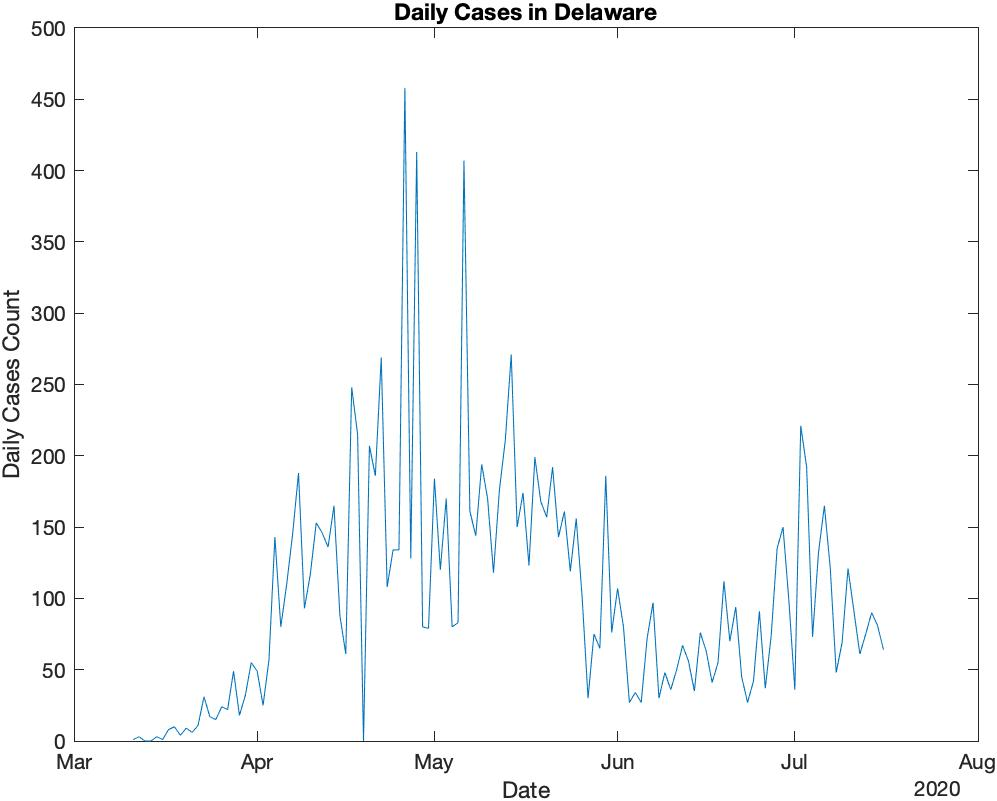
\includegraphics[width=0.43\textwidth]{Figure3a.jpg}%
    \label{fig:a}%
  }%
  \hfill
  \subfigure[b]{%
    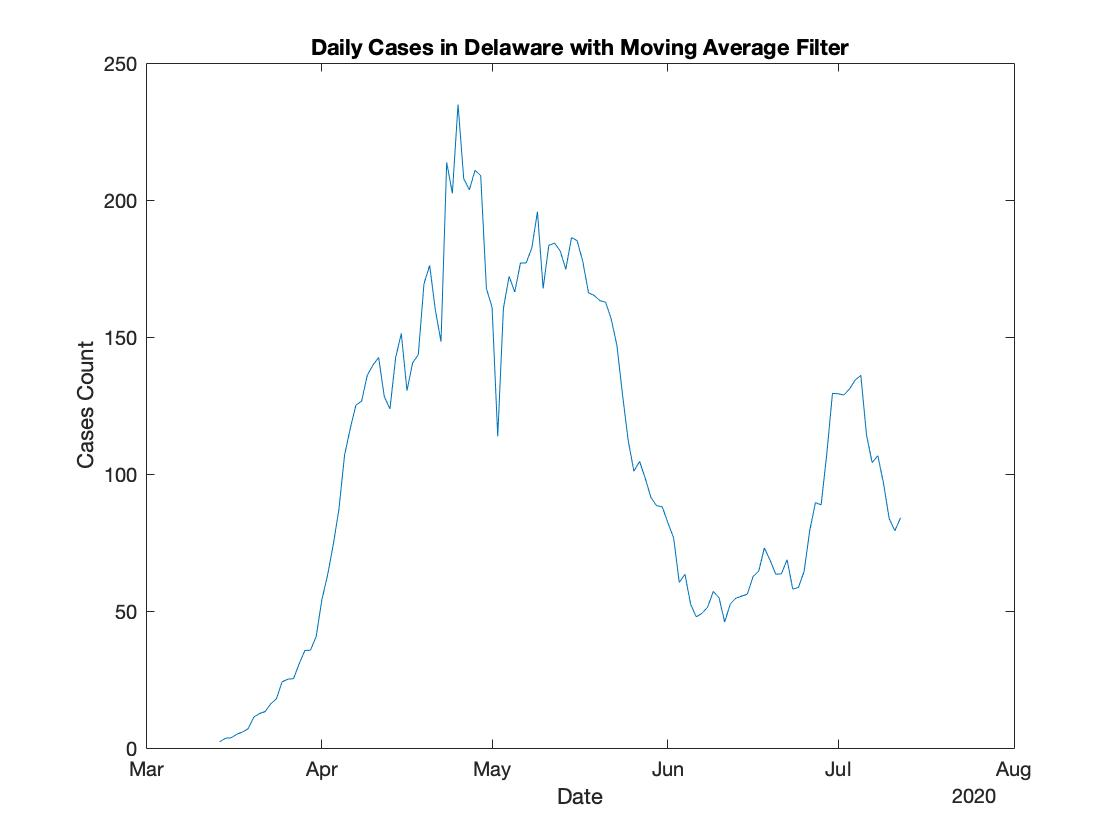
\includegraphics[width=0.5\textwidth]{Figure3b.jpg}%
    \label{fig:b}%
  }%
  \caption{The scatter plot A shows the extreme variance found in the daily counts of COVID-19 cases in Delaware. As can be expected, the moving average filter of 7-days creates a smoother plot and makes the data appropriate for fitting to a model.}
  \label{fig:4}
\end{figure}
\paragraph{} After creating this dataset composed of daily data with a moving average filter, it was possible to begin the data fitting procedure. The procedure is similar to that of Cumulative Data: $y = ae^{kt}$. There are 14-day modeling windows, and the data is fitted by linearizing the function and solving for the parameters that result in the shortest distance between the real data and the model, a least squares fit. As was done before, this calculation also had a bootstrapping procedure where random samples with replacement were taken from the data and sent to data fitting 1000 times. The mean was accepted as the calculated parameter value and the 25th and 975th values as the lower and upper bounds, respectively.
\paragraph{} The second model, $y = ae ^ {kt} + b$, was attempted on the daily data but found to be inappropriate for this dataset. The calculations for the parameters did not work because nearly all the modeling windows had the same $k$ throughout the entire program. The reason for the daily data not requiring the additional $+b$ parameter is because of how the data was calculated. Since it was calculated by subtracting the one day from the previous, the following assumption results: if $y_{n+1} = ae^{k(t+1)} + b$ and $y_{n} = ae^{kt} + b$, then the result is a value that effectively nullifies $b$ because there should not be extreme changes in b from one modeling window to the next. Because of this, daily data was only modeled with $y = ae^{kt}$. As previously stated, the methods for this are the same as the $y = ae^{kt}$ model for the cumulative data except for the addition of the moving average filter.
\paragraph{} As of July 18th, 2020 there were 110 modeling windows in this analysis. These calculations are reflected in \href{https://github.com/tatabas/delaware-covid-analysis}{finalDailyDelaware.m}.

\section{Analysis \& Application}
\subsection{The Daily Data}
To begin applying the quantitative trends in the graphics to real events in Delaware, some markers were added to dates of importance. These figures display the data for the daily cases data that were analyzed:

\begin{figure}[h]
  \centering
  \subfigure[a]{%
    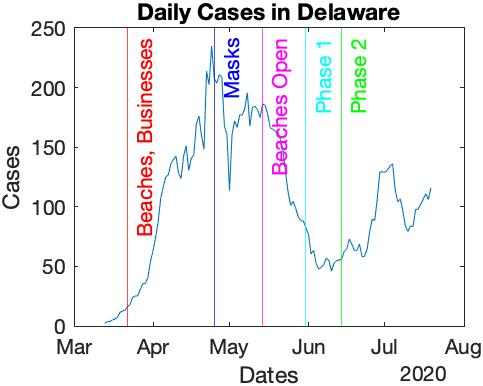
\includegraphics[width=0.3\textwidth]{Figure4a.jpg}%
    \label{fig:a}%
  }%
  \hfill
  \subfigure[b]{%
    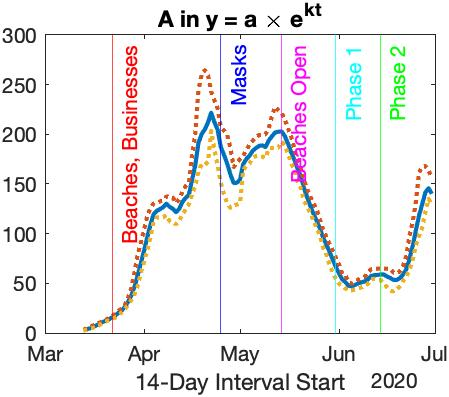
\includegraphics[width=0.3\textwidth]{Figure4b.jpg}%
    \label{fig:b}%
  }%
  \hfill
  \subfigure[c]{%
    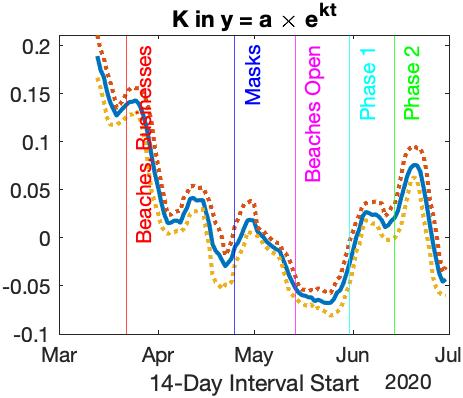
\includegraphics[width=0.3\textwidth]{Figure4c.jpg}%
    \label{fig:b}%
  }%
  \caption{Daily cases data were modeled in 14-day windows to the equation $y=ae^{kt}$. The 95\% Confidence are shown with the red and yellow dotted lines for each parameters $k$ and $a$. The other lined markers display the following information:}
  \label{fig:3}
\end{figure}

\begin{itemize}
  \item Red Line: "Beaches Businesses", March 22
  \item Blue Line: "Masks", April 25
  \item Purple Line: "Beaches Open", May 14
  \item Cyan Line: "Phase 1", May 31
  \item Green Line: "Phase 2", June 14
\end{itemize}

\paragraph{}For the remainder of the discussion on how these calculations relate to the real events in Delaware, most -- if not all -- the attention will be turned to the $k$ parameter. The most important parameter is $k$ in that it defines the exponential growth. If $k$ is positive, we have exponential growth, and the larger the $k$, the more severe rate of infection there is. If $k$ is negative, then the virus is in decline. Because the 14-day window is moved down one day, it is possible to closely monitoring $k$ and relate it to events in the state.

\paragraph{} The first incline in k values comes around March 20, making a parabolic shape, then dropping back down into a decline. This is an interesting point because is coincides with many activities in Delaware. First, during this time period there were outbreaks within nursing homes, which became very severe during March and early April. However, also worth noting, is the weekend starting with March 20th. During this weekend, there was a \href{https://www.delmarvanow.com/story/news/local/delaware/2020/03/20/rehoboth-beach-draws-crowds-despite-coronavirus-threat-delaware/2887892001/}{news article^6} that outlines the immense crowding of Delaware beaches on March 20th. Together, the nursing homes and crowding of beaches, caused rises in cases throughout Delware in the late March time period.
\paragraph{} In response to the nursing home outbreaks, the State of Delaware offered closely monitored policies specifically for nursing homes that were updated with frequency in the early days of the pandemic. These policies ranged from isolation to limiting visitors, to also defining how residents should be brought back to the facility after successful treatment. Since nursing homes had become one of the epicenters of the virus in Delaware, these precautions were necessary and rightfully taken. The policies aimed specifically at nursing homes seem to have worked in starting a steady decrease in the $k$ value following March 27th.

\begin{figure}[h]
  \centering
    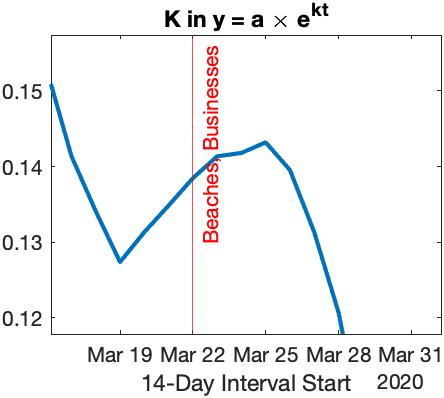
\includegraphics[width=0.3\textwidth]{Figure5.jpg}%
    \label{fig:a}%
  \caption{The K parameter from modeling the daily cases data of COVID-19 in Delware to $y=ae^{kt}$ in 14-day windows zoomed into the time period that relates to nursing homes and crowded beaches. The red line with beaches, businesses marks the date that beaches and non-essential businesses were forced to close.}
  \label{fig:5}
\end{figure}

\paragraph{} To measure the impact of the crowded beaches, it is important to note the incubation time of the virus.  It was found in a study that it takes \href{https://pubmed.ncbi.nlm.nih.gov/32150748/}{approximately 5 days^6} to develop the first symptoms of the virus. Therefore, adding 5 days after each major incidence should align with the a logical conclusion in the rises or falls of the $k$ parameter. If March 20th is taken as an exposure date for individuals that were in the crowd and possibly contracted the virus, adding 5 days results in March 25th, which is the peak of the parabolic increase in the $k$ parameter. Since 5 days following exposure is located at the peak of the curve, it is reasonable to assume that the beaches were not the only factor in this mini-outbreak. Mixed with the effects of the outbreaks in nursing homes, the crowded beaches created this mini-outbreak, which then falls. The fall can be attributed to Delaware's speedy responses to these situations. overnor Carney issued orders to close Non-Essential businesses and both public and private beaches just two days after the incident on March 20th. With the closure of non-essential businesses, and regulations in essential business, the $k$ parameter had a successful decline.

\paragraph{}This decline is then interrupted by another parabolic increase in $k$ values in early- to mid-April. Although other factors could have come into play, this mini-outbreak can be attributed to the chicken factories in Sussex County. It was \href{https://www.foxnews.com/food-drink/delaware-chicken-company-attendance-kill-chickens-coronavirus}{reported^8} on April 15th that the chicken factories were suffering from employee shortages. Since employees were already diagnosed and dismissed from the factories by this date, there is no need to add 5 days to calculate the exposure to symptomatic period.

\begin{figure}[h]
  \centering
  \subfigure
    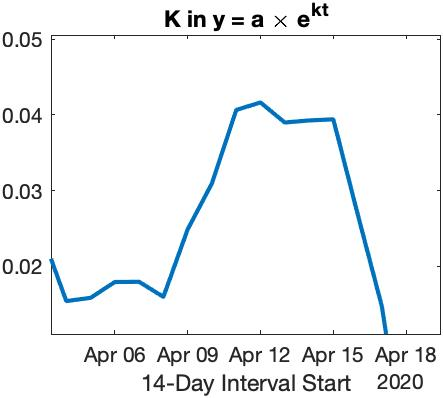
\includegraphics[width=0.4\textwidth]{Figure6.jpg}%
    \label{fig:a}%
  \caption{The K parameter from modeling the daily cases data of COVID-19 in Delware to $y=ae^{kt}$ in 14-day windows zoomed into the time period that relates to chicken factory outbreaks.}
  \label{fig:6}
\end{figure}

\paragraph{} After the chicken factory outbreak period the $k$ value changes in many unusual ways. However, since this portion of the data exists in the crossing between a positive and negative $k$ value, it should be taken with a grain of salt. Especially in some points within this period of mid-April, the 95\% confidence interval, marked with the red and yellow dotted lines, include the point 0. If the confidence interval includes 0, there is a chance that the virus is not growing in infection rate at all, which is good. This shows that the collective effects of the policies helped curb the spread of the virus and control the pandemic. This critical interval is an important transition period that the model used here may not capture with accuracy. Since it is transitioning from an infective rate to a declining rate, the transition may cause higher rates of uncertainty. This uncertainty can be seen with the width of the confidence intervals but also with the least squares errors, as shown in Figure 7.

\paragraph{} During the period of uncertainty in the model, it is unknown in this study whether the quick increase is a continuation of the chicken factory outbreak or another source. Whatever the cause, the $k$ values were showing a quick and rapid rise that continued through April 29th. During this rise, the $k$ values marked with blue are negative, but the confidence interval includes positive values. At this point, the virus is transition between an infective and declining nature. However, the real cases do keep on rising. There were 161 more cases reported on April 23rd. Governor Carney introduced a universal masking requirement for people in Delaware on April 25th. This fast response helped with preventing a further increase in infectivity. 5 days after this requirment, the $k$ values starts to create a local maxima and begins to fall again.

\begin{figure}[h]
  \centering
  \subfigure[a]{%
    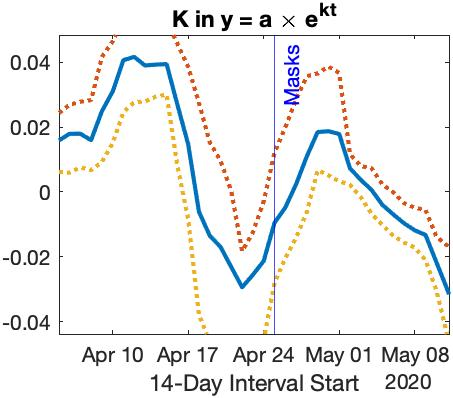
\includegraphics[width=0.3\textwidth]{Figure7.jpg}%
    \label{fig:a}%
  }%
  \hfill
  \subfigure[b]{%
    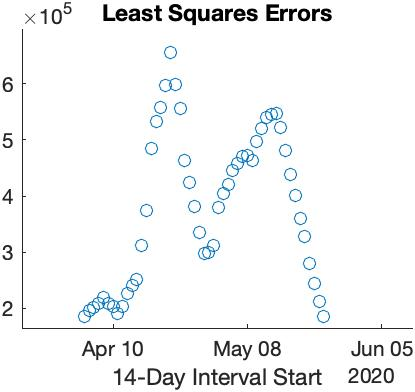
\includegraphics[width=0.3\textwidth]{Figure7a.jpg}%
    \label{fig:b}%
  }%
  \caption{The K parameter from modeling the daily cases data of COVID-19 in Delware to $y=ae^{kt}$ in 14-day windows zoomed into the time period that relates to chicken factory outbreaks in 7a. and the corresponding least squares errors in 7b. The blue line in 7a labeled Masks is the date, April 25th, which a universal requirment of masks were required for people in Delaware.}
  \label{fig:7}
\end{figure}

In order to further explore the instances in this period, a simple rate of change calculation between each $k$ value was performed (a simple slope calculation). Even though the calculations are very rapidly changing and do not appear to show a smooth transitions, it portrays that idea that the $k$ parameter changes from a decreasing trend to positive trend up to April 29th, where the rate of change of $k$ is close to 0. This indicates that the $k$ value is going back to a decreasing mode starting April 30th. The universal, required masking helped control the spread of the virus.

\begin{figure}[h]
  \centering
  \subfigure
    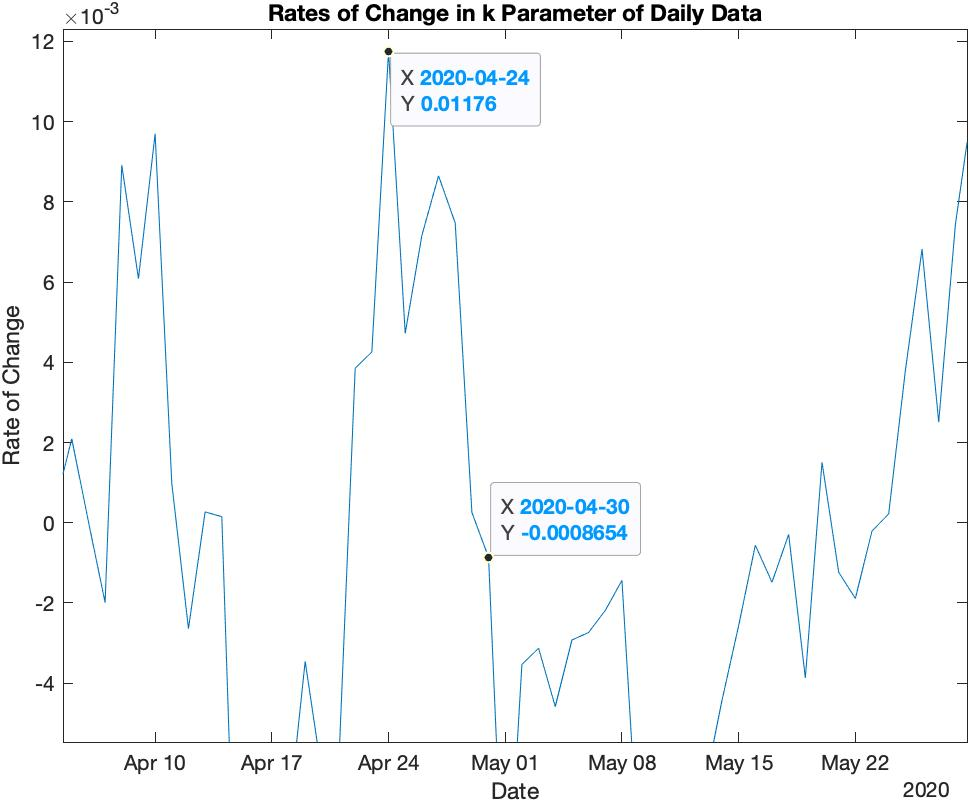
\includegraphics[width=0.4\textwidth]{Figure8.jpg}%
    \label{fig:a}%
  \caption{A simple rate of change calculation between each $k$ value in the form of $\frac{(k+1)-k)}{((x+1)-x)}$. This was applied to the $k$ values obtained from the 14-window modeling on daily data for the $y=ae^{kt}$ equation. }
  \label{fig:8}
\end{figure}

In effort to compare the the effects of the closing beaches and non-essential businesses with a masking requirement, these intervals will be split into phases. This method was inspired by another study conducted in the \href{https://jamanetwork.com/journals/jama/fullarticle/2768533}{MassGen Boston hospitals^9}. The date of closures were taken as the beginning, then there were 5 days added on to wait for the virus to show up in the data as cases. This phases ended before the mini-outbreak starts, so the time frame in consideration is March 27th to April 4th. To calculate the line here, a simple slope formula of $y = mx + b$ was used. The slope for this period was -0.0145. The same process was applied to masking and the slop was -0.0051. Even though this calculation is by no means complex and comprehensive, it shows that logical relation that keeping people in their homes has a greater impact on controling the spread of the virus. If a greater percentage of people are sheltering in their homes, then the susceptible population does not get the virus because susceptible and infectious individuals are all in their homes, limiting interaction.

\begin{figure}[h]
  \centering
  \subfigure[a]{%
    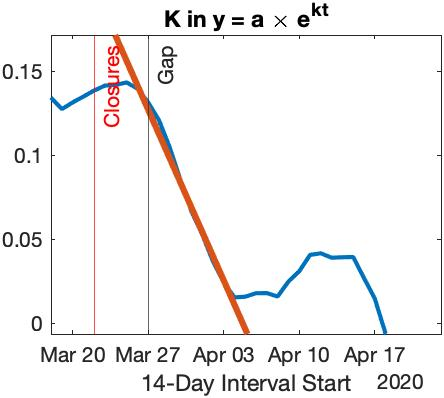
\includegraphics[width=0.3\textwidth]{Figure9a.jpg}%
    \label{fig:a}%
  }%
  \hfill
  \subfigure[b]{%
    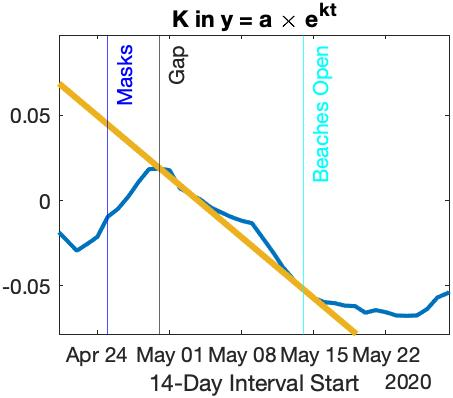
\includegraphics[width=0.3\textwidth]{Figure9b.jpg}%
    \label{fig:b}%
  }%
  \caption{For Figure 9a a line of form $y = -0.0145x+0.33$ is overlayed on the $k$ values calculated from the daily cases COVID-19 data through the 14-day modeling window for the equation $y=ae^{kt}$. Figure 9a expresses the effect of beach and business closures. The same was done for the Figure 9b that shows the effects of required masking. The line is of form $y=-0.0051x+0.264$}
  \label{fig:9}
\end{figure}

\paragraph{} After beaches start to open up again, the rate of decrease goes down, as can be seen visually by the rounding of the decline and the change to an inclined rate of change occurring after the beaches open up. The portion of data following the opening of beaches has many activities that can cause an increase in the spread of the virus. The State of Delaware had very specific guidelines for opening up the beaches to ensure distancing and safety, but there is only so much the State can do. Of course, it cannot be taken out of consideration that if it were not for these precautions, the spread of the virus could have been worse. However, it is impossible to ignore the fact that even without the precautions there was an increase in the spread of the virus.

\paragraph{} Another event that could have accelerated the spread of the virus, and can possibly explain the increase of the $k$ values in late May, are the George Floyd protests that erupted across the country. Delaware was no exception. From the data available in this study, it is impossible to pin-point the effects of the protests or the relaxation of the quarantine on the increase of $k$. It can be reasonably assumed that the two acted together.

\begin{figure}[h]
  \centering
  \subfigure
    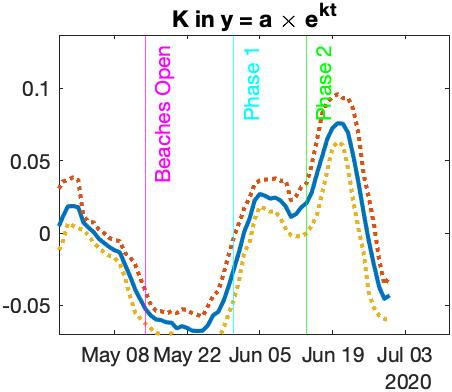
\includegraphics[width=0.4\textwidth]{Figure10.jpg}%
    \label{fig:a}%
  \caption{The K parameter from modeling the daily cases data of COVID-19 in Delware to $y=ae^{kt}$ in 14-day windows zoomed into the time period that relates to final portions of the analyzed data.}
  \label{fig:10}
\end{figure}

\paragraph{} With the introduction of phased openings, many business sectors saw increased legislation on their business operations. Many were for good reason, helping businesses open and restart the economy in a responsible and safe way. The effects and specificity in the documents pertaining to each type of business is truly commendable. Also, Phase 1 openings do not seem to play a big role in an increase or decrease of $k$. By applying the 5-day gap, it is possible to see that the Phase 1 effective period (the period when its effects can be measured) correllates with the peak of the previous incline. This could possibly indicate that with more experience in applying distancing measures on beaches, and with the decrease of the protests, the infection rate was decreasing. The enforcement of controlled social interactions do make an impact.

\paragraph{} The story is a bit different with Phase 2. With more establishments opening up, and the susceptible populations being more prone to interactions with a member of the infectious population. this is inevitable. The important part is controlling the growth, which the State of Delaware did -- and continues to do -- very well. Each outbreak was followed by timely and proper policies that helped combat the threat of increased transmission.

\paragraph{} The good news from the visual is that the $k$ value peaks and then drops. This drop may be associated with the fact that Delawre enacted further measures that modified the Phase 2 opening plans. For example, it was seen that bars were acting as a major hotspot for transmission, so further regulations were put in place for bars and their taprooms. Further limitations and sanitary requirements were placed for indoor and outdoor dining. All of these in concert help create an environment where transmission is decreased and the spread of the virus is controlled.


\subsection{The Cumulative Data}
After getting a sense of the trends in the State with the daily date, it is worth taking a note at the cumulative data. In this analysis, it is again important to look at the $k$ values since this is the exponential parameter that reflects the extent of the virs spreading. Moreover, since the cumulative data was based on the model $y=ae^{kt} +b$ it is important to study the impact in b, since this should express another view on the extent of the increases or decreases in the cases as policies change.

\begin{figure}[h]
  \centering
  \subfigure
    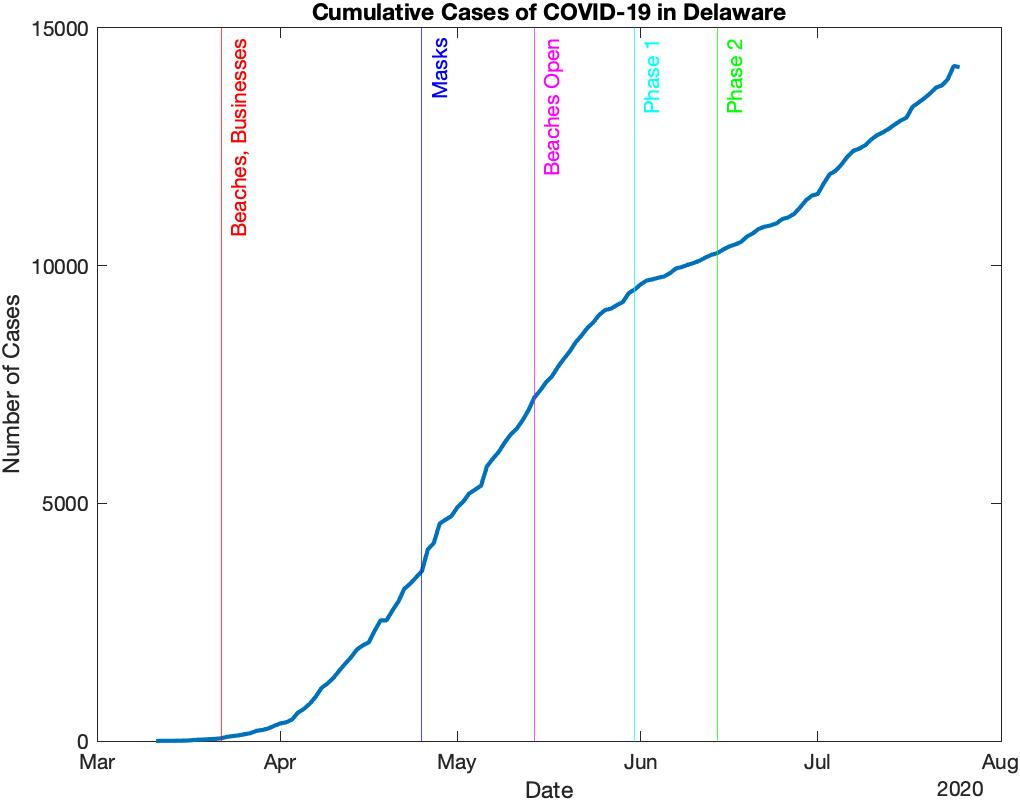
\includegraphics[width=0.3\textwidth]{Figure11.jpg}%
  \caption{The untouched data of cumulative COVID-19 cases in Delaware. The same markings from before are used to show when policies were enacted.}
  \label{fig:10}
\end{figure}

\paragraph{} Of course, because the data in this set is of cumulative cases, there will never be a negative exponential growth. A decrease of positivity in $k$ will be accepted as a decrease in the spread of the virus. In many instances, the conclusions that were made with the previous model can also be made with this model on cumulative data. For example, the first outbreak that was associated with nursing homes and beaches, and the second outbreak associated with chicken factories also show up in this model.

\begin{figure}[h]
  \centering
  \subfigure[a]{%
    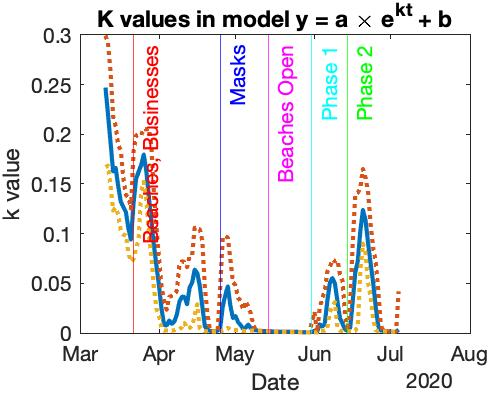
\includegraphics[width=0.3\textwidth]{Figure12a.jpg}%
    \label{fig:a}%
  }%
  \hfill
  \subfigure[b]{%
    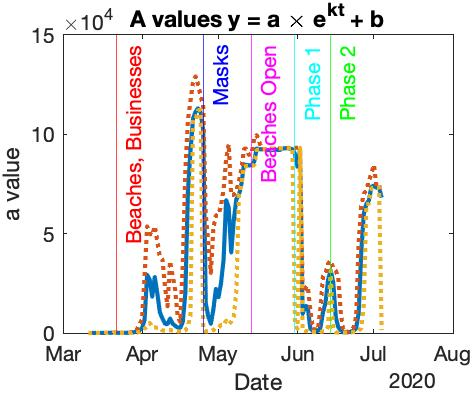
\includegraphics[width=0.3\textwidth]{Figure12b.jpg}%
    \label{fig:b}%
  }%
  \hfill
  \subfigure[c]{%
    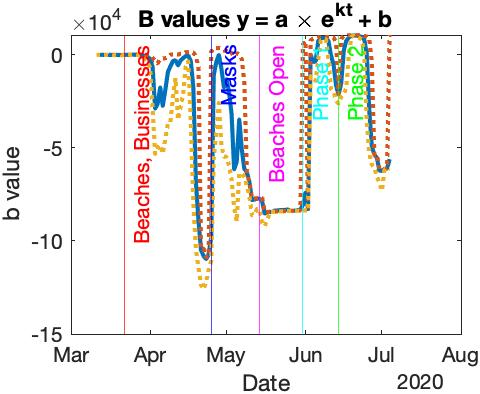
\includegraphics[width=0.3\textwidth]{Figure12c.jpg}%
    \label{fig:b}%
  }%
  \caption{Cumulative COVID-19 cases data were modeled in 14-day windows to the equation $y=ae^{kt}+b$. The 95\% Confidence are shown with the red and yellow dotted lines. The parameters of $k$, $a$, and $b$ are shown here. The other lined markers display the following information:}
  \label{fig:12}
\end{figure}
\begin{itemize}
  \item Red Line: "Beaches Businesses", March 22
  \item Blue Line: "Masks", April 25
  \item Purple Line: "Beaches Open", May 14
  \item Cyan Line: "Phase 1", May 31
  \item Green Line: "Phase 2", June 14
\end{itemize}

\paragraph{} The same conclusions can be made about these outbreaks since the increasing parabolic trends and subsequent decreases are all shaped in a similar fashion. Even though this is true, it is worth taking a look at the late May interval where the virus seemed to have a transition period and there was uncertainty in the previous model.

\paragraph{} This portion of the model in the cumulative model shows the same trend: following the chicken factories outbreak, there is a sudden drop. This is probably due to the fact that this was a localized outbreak and did not ripple throughout the rest of Delaware. Then, there is a sudden rise, which is curtailed by the Masking requirement. The masking requirements effects are again seen in following April 20th as both the $k$ values and $b$ values fall. The $b$ value solidifies the chicken factory outbreak as a more isolated event because the $b$ value is high during the outbreak due to rapid increases in the number of cases. Then, after the outbreak the $b$ value falls rapidly. Since the cases in the factories were controlled, the rapid decrease in the number of cases caused an large change in the model.

\begin{figure}[h]
  \centering
  \subfigure[a]{%
    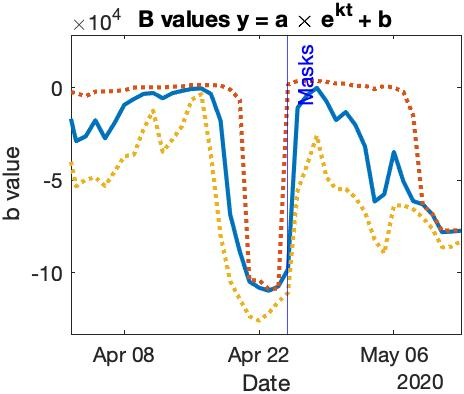
\includegraphics[width=0.3\textwidth]{Figure13a.jpg}%
    \label{fig:a}%
  }%
  \hfill
  \subfigure[b]{%
    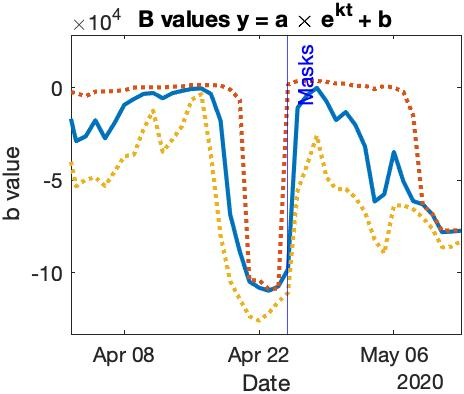
\includegraphics[width=0.3\textwidth]{Figure13b.jpg}%
    \label{fig:b}%
  }%
  \caption{Cumulative COVID-19 cases data were modeled in 14-day windows to the equation $y=ae^{kt}+b$. The 95\% Confidence are shown with the red and yellow dotted lines. This figure focuses on the interval during the chicken factory outbreak and after.}
  \label{fig:13}
\end{figure}

\paragraph{} The $b$ parameter is also appropriate to further commend the usage of masking in Delaware. As was explained in the daily data, masking did cause a decrease in the $k$ parameter. The same pattern is reflected in the cumulative data, so this will not be explained again. Moreover, masking's effects can also be shown in the $b$ parameter. 5 days after masking, the $b$ parameter falls to negative values. This shows a decrease in the exponential model of the cases: the exponential rate of growth is in decline. Even if masking was not the only factor, it does play a role in controling the spread of the virus.

\paragraph{} In efforts of comparing the last few policy intervals, the daily data graphic is reintroduced with the cumulative data:
\begin{figure}[h]
  \centering
  \subfigure[a]{%
    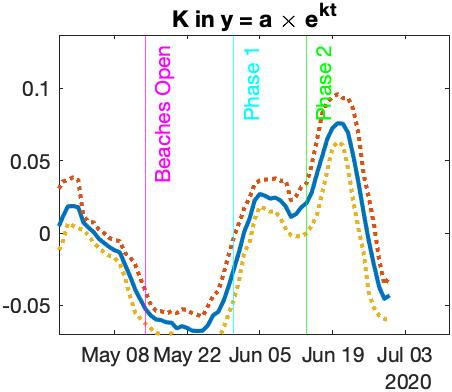
\includegraphics[width=0.3\textwidth]{Figure10.jpg}%
    \label{fig:a}%
  }%
  \hfill
  \subfigure[b]{%
    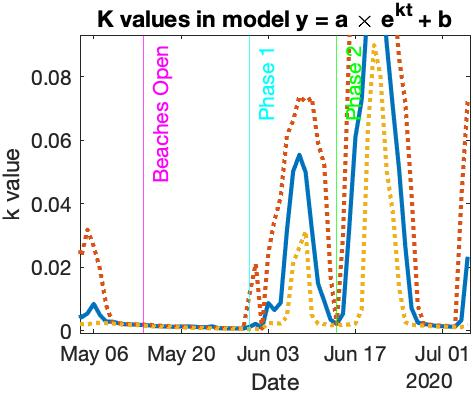
\includegraphics[width=0.3\textwidth]{Figure14b.jpg}%
    \label{fig:b}%
  }%
  \subfigure[c]{%
    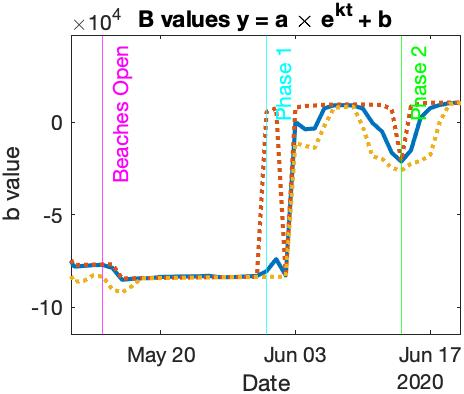
\includegraphics[width=0.3\textwidth]{Figure14c.jpg}%
    \label{fig:a}%
  }%
  \caption{Figure 14a is the same graphic from Figure 10. This shows the $k$ values calculated from the daily data modeled in 14-day windows for the equation $y=ae^{kt}$. The red and yellow dotted lines are the upper and lower limites of the 95\% confidence interval. Figures 14b and 14c show a similar time interval with for the cumulative data modeled in 14-day windows for the equation $y=ae^{kt}+b$. The red and yellow dotted lines are the upper and lower limites of the 95\% confidence interval.}
  \label{fig:14}
\end{figure}

\paragraph{} The decline in the exponential parameters after masking results in a flat-line for the $k$ and $b$ values in the cumulative data examples. Whereas, the daily data example is a gradual fall. This could mean that the $+b$ parameter is not appropriate for this time interval. The decrease in decline, but still decay of the virus growth rate after beaches open, as observed in the daily data example, is more logically sound. Comparing the two models is important because one model may capture one event while the other does not.

\paragraph{} The rest of the events follow the same patterns as the daily data. An increase between Phase 1 and Phase 2 that later falls. Then an increase between after Phase 2 that also falls. With the information available during this study, this fall after Phase might be attributed to Governey Carney's response to bars and taprooms, as well as restaurants.

\subsection{Conclusion}
\paragraph{} The overall theme in the association of the data and graphics with the policies lies in the fact of control. Delaware had timely responses to each of the outbreaks that occurred in the State during the pandemic. Each of these responses were successful in their own way. Some responses came within days, as with the overcrowded beaches example: the response to close beaches came just 2 days after the incident. This timely behavior by the policy makers of Governer Carney's office and the State of Delaware truly did help control the spread and help the State of Delaware. Most of the outbreaks were from isolated events like the nursing homes and chicken factories. The state itself was put under control with shelter-in-place and state of emergency orders that included and was not limited to closing businesses and requiring masks. These have profound effects that were displayed in two models looking at Cumulative and Daily COVID-19 cases in Delaware.

\section{Acknowledgments}
\paragraph \noindent I would like to thank Professor Piovoso from the Engineering Department at Swarthmore College for his support and mentorship during this project. I would also like to thank the \href{https://www.swarthmore.edu/summer-research-opportunities/natural-sciences-and-engineering}{Swarthmore College donors^{10}} for making this project possible. Additional recognition is given to the New York Times for uploading COVID-19 cases data to their \href{https://github.com/nytimes/covid-19-data/blob/master/us-states.csv}{GITHUB Repository}.

\pagebreak
\section{References}
\begin{enumerate}
  \item Record of Delaware Actions: \\\url{https://governor.delaware.gov/health-soe/}
  \item New York Times COVID-19 Cases Data: \\\url{https://github.com/nytimes/covid-19-data/blob/master/us-states.csv}
  \item MATLAB fmincon Function:\\ \url{https://www.mathworks.com/help/optim/ug/fmincon.html}
  \item My GITHUB Repository:\\ \url{https://github.com/tatabas/delaware-covid-analysis}
  \item MATLAB Bootstrap Function: \\\url{https://www.mathworks.com/help/stats/bootstrp.html}
  \item News Article about March 20: \\\url{https://www.delmarvanow.com/story/news/local/delaware/2020/03/20/rehoboth-beach-draws-crowds-despite-coronavirus-threat-delaware/2887892001/}
  \item Study outlining the incubation of the virus:\\ \url{https://pubmed.ncbi.nlm.nih.gov/32150748/}
  \item Chicken Factory news: \\ \url{https://www.foxnews.com/food-drink/delaware-chicken-company-attendance-kill-chickens-coronavirus}
  \item MassGen study: \\
  \url{https://jamanetwork.com/journals/jama/fullarticle/2768533}
  \item Swarthmore College Summer Research Program: \\\url{https://www.swarthmore.edu/summer-research-opportunities}
\end{enumerate}}

\end{document}
